\documentclass[10pt,leter,openany]{article}
\usepackage[latin1]{inputenc}
\usepackage[english]{babel}
\usepackage{amsmath}
\usepackage{amsfonts}
\usepackage{amssymb}
\usepackage{graphicx}
\usepackage{listings}
\usepackage{color}
\usepackage[left=3cm,right=3cm,top=3cm,bottom=3cm]{geometry}
\usepackage[numbers,sort&compress]{natbib}
\usepackage{url}
\usepackage{caption}
\usepackage{siunitx}
\usepackage{subfigure}
\usepackage{float}
\usepackage{booktabs}

\usepackage{comment}

\setlength{\parindent}{0pt}
\setlength{\parskip}{4pt}

\definecolor{mygreen}{rgb}{0,0.6,0}
\definecolor{mygray}{rgb}{0.5,0.5,0.5}
\definecolor{mymauve}{rgb}{0.58,0,0.82}

\lstset{ 
	backgroundcolor=\color{white},   % choose the background color; you must add \usepackage{color} or \usepackage{xcolor}; should come as last argument
	basicstyle=\footnotesize,        % the size of the fonts that are used for the code
	breakatwhitespace=false,         % sets if automatic breaks should only happen at whitespace
	breaklines=true,                 % sets automatic line breaking
	captionpos=b,                    % sets the caption-position to bottom
	commentstyle=\color{mygreen},    % comment style
	deletekeywords={...},            % if you want to delete keywords from the given language
	escapeinside={\%*}{*)},          % if you want to add LaTeX within your code
	extendedchars=true,              % lets you use non-ASCII characters; for 8-bits encodings only, does not work with UTF-8
	firstnumber=01,                	 % start line enumeration with line 1000
	frame=single,	                 % adds a frame around the code
	keepspaces=true,                 % keeps spaces in text, useful for keeping indentation of code (possibly needs columns=flexible)
	keywordstyle=\color{blue},       % keyword style
	language=Python,                 % the language of the code
	morekeywords={*,...},            % if you want to add more keywords to the set
	numbers=left,                    % where to put the line-numbers; possible values are (none, left, right)
	numbersep=5pt,                   % how far the line-numbers are from the code
	numberstyle=\tiny\color{mygray}, % the style that is used for the line-numbers
	rulecolor=\color{black},         % if not set, the frame-color may be changed on line-breaks within not-black text (e.g. comments (green here))
	showspaces=false,                % show spaces everywhere adding particular underscores; it overrides 'showstringspaces'
	showstringspaces=false,          % underline spaces within strings only
	showtabs=false,                  % show tabs within strings adding particular underscores
	stepnumber=1,                    % the step between two line-numbers. If it's 1, each line will be numbered
	stringstyle=\color{mymauve},     % string literal style
	tabsize=2,	                     % sets default tabsize to 2 spaces
	title=\lstname                   % show the filename of files included with \lstinputlisting; also try caption instead of title
}

\usepackage{titling}
\newcommand{\subtitle}[1]{%
	\posttitle{%
		\par\end{center}
	\begin{center}\large#1\end{center}
	\vskip0.5em}%
}


\author{5273}
\title{Homework Assignment 2: Applied Probabilistic Models}
\subtitle{Analysis of the Book Structure}
\date{}



\begin{document}
	
\maketitle

\section{Introduction}
	
	For this work, data is collected on the free eBooks library Project Gutenberg \cite{gutenberg}. The chosen book for the analysis is: ``The Autobiography of Benjamin Franklin". Data obtained from the Project Gutenberg are in \texttt{txt} format.
	
	For the analysis, it is used the R software in its version 4.0.2 \citep{r}, and the code used is available on the GitHub repository \citep{github}. This work is run on a MacBook Air with an Intel Core i5 CPU $ @ $ 1.8 GHz and 8 GB RAM.
	
\section{Data}
	 
	The book is downloaded directly from the web and in order to develop the analysis, the following code is used.
	
	\lstinputlisting[language=R, firstline=1, lastline=8]{a2.R}
	
	The book has a total of 294 003 characters (letters) and 66 520 words. This data is used to a further analysis of what the most important letters and words are according to its frequency. The next part of the code is set to this objective.
	
\newpage

	\lstinputlisting[language=R, firstline=10, lastline=61]{a2.R}


\subsection{Letters}
	For the analysis of the letters, barplots are generated. Here the horizontal axis represents all the used letters and the vertical one the corresponding frequencies. Figure \ref{fig:barplot_letters} shows in (a) all the letters present in the document, sorted in decreasing order and by the same token in (b)  it can be seen the most used letters. In this latter case frequency greater than 500 is the criteria to fall in this category.  Frequencies of the six most used letters are shown in Table \ref{tab:my-table1}. 

	
	\begin{figure}

		\centering
		\subfigure[Barplot of all letters present in the document]{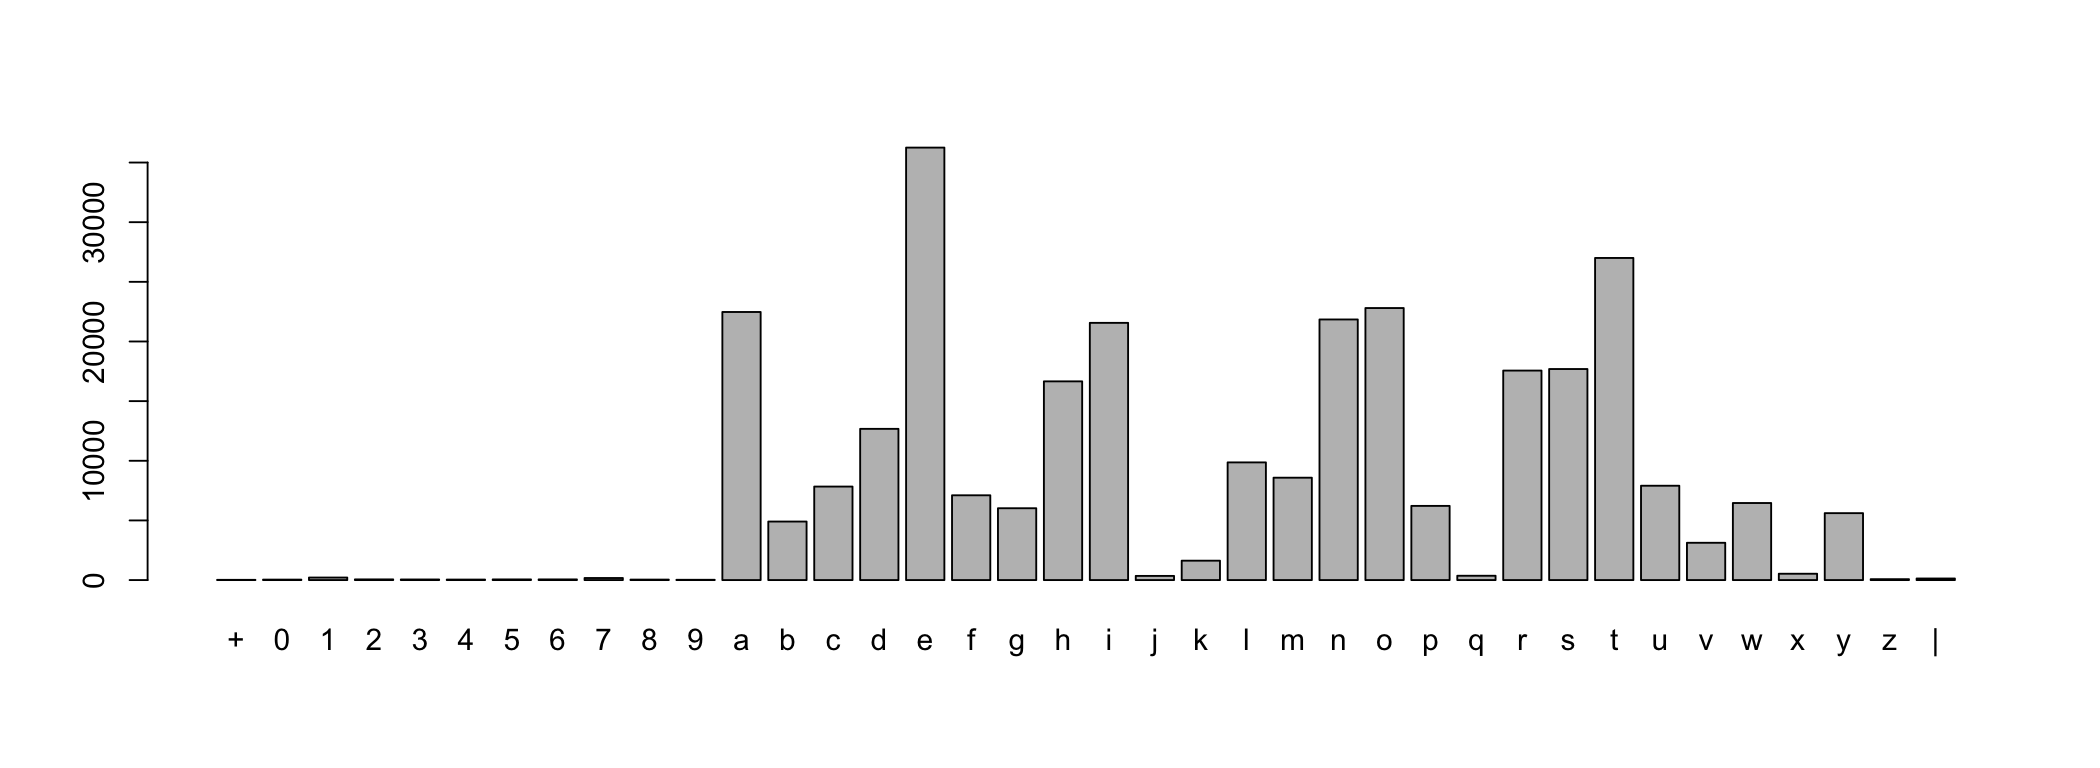
\includegraphics[width=170mm]{img/barplot_letters}}
		\subfigure[Barplot of most used letters]{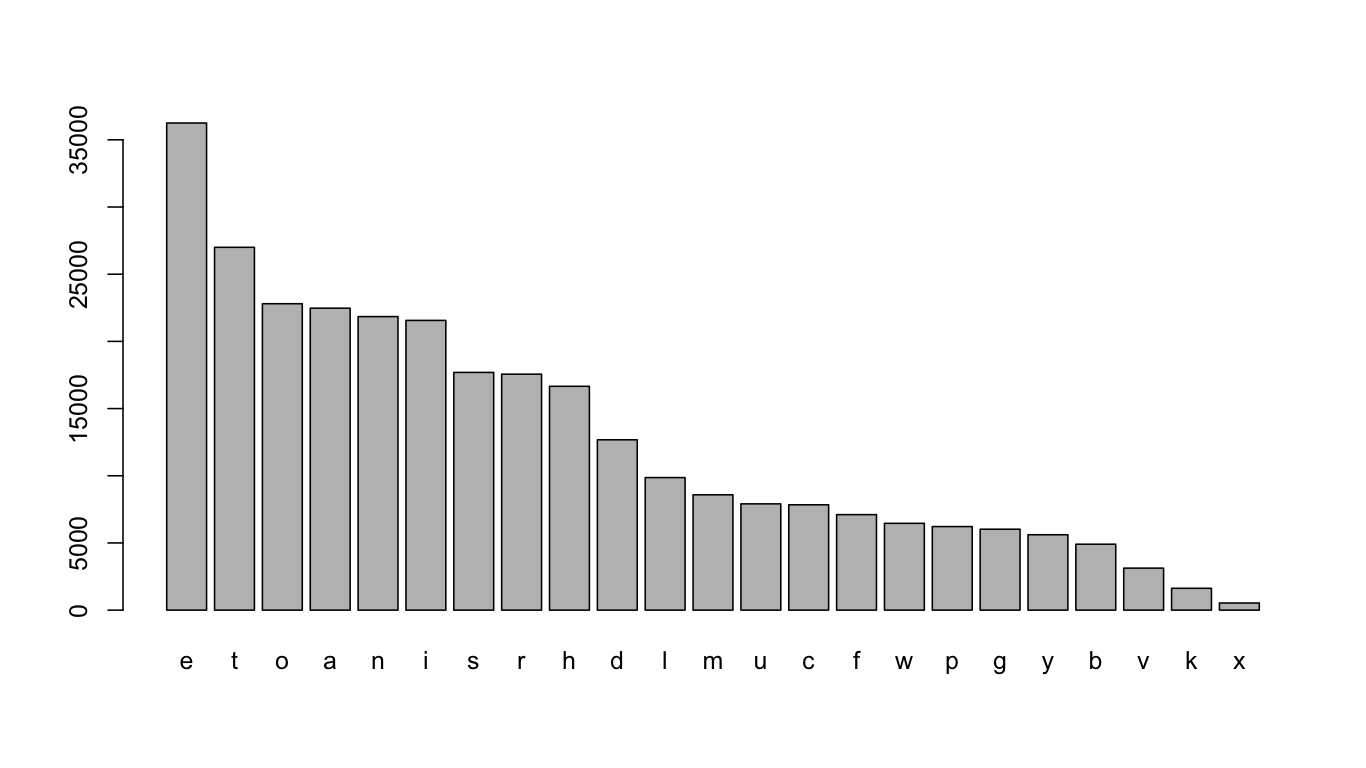
\includegraphics[width=120mm]{img/barplot_relevant_letters_ordered}}
		
		\caption{Barplots of letters present in the document} \label{fig:barplot_letters}

\end{figure}

% Please add the following required packages to your document preamble:
% \usepackage{booktabs}
\begin{table}[]
	\centering
	\caption{Frequency of most used letters}
	\label{tab:my-table1}
	\begin{tabular}{@{}ll@{}}
		\toprule
		Letter & Frequency \\ \midrule
		e      & 36 252    \\
		t      & 27 001    \\
		o      & 22 803    \\
		a      & 22 472    \\
		n      & 21 845    \\
		i      & 21 561    \\ \bottomrule
	\end{tabular}
\end{table}

\newpage

\subsection{Words}	
	In a similar fashion, barplots are generated for the analysis of words. Here the horizontal axis represents all the used words in the document and the vertical one corresponds to the respective frequencies.

	In the first attempt, it is hard to see a difference among words, that is why the following barplots are generated. Figure \ref{fig:barplot_words1} shows the words filtered. In (a)  it can be seen the frequency of the most used words. For this category, it is set as a requirement a frequency greater than 100. Furthermore, in (b), for this category, it is discarded the words with a frequency greater than 250 because articles and prepositions are included and these words are not very descriptive. Finally, those relevant words are sorted in decreasing order in Figure \ref{fig:barplot_words2}.

		\begin{figure}
		\centering
		\subfigure[Barplot of most used words present in the document]{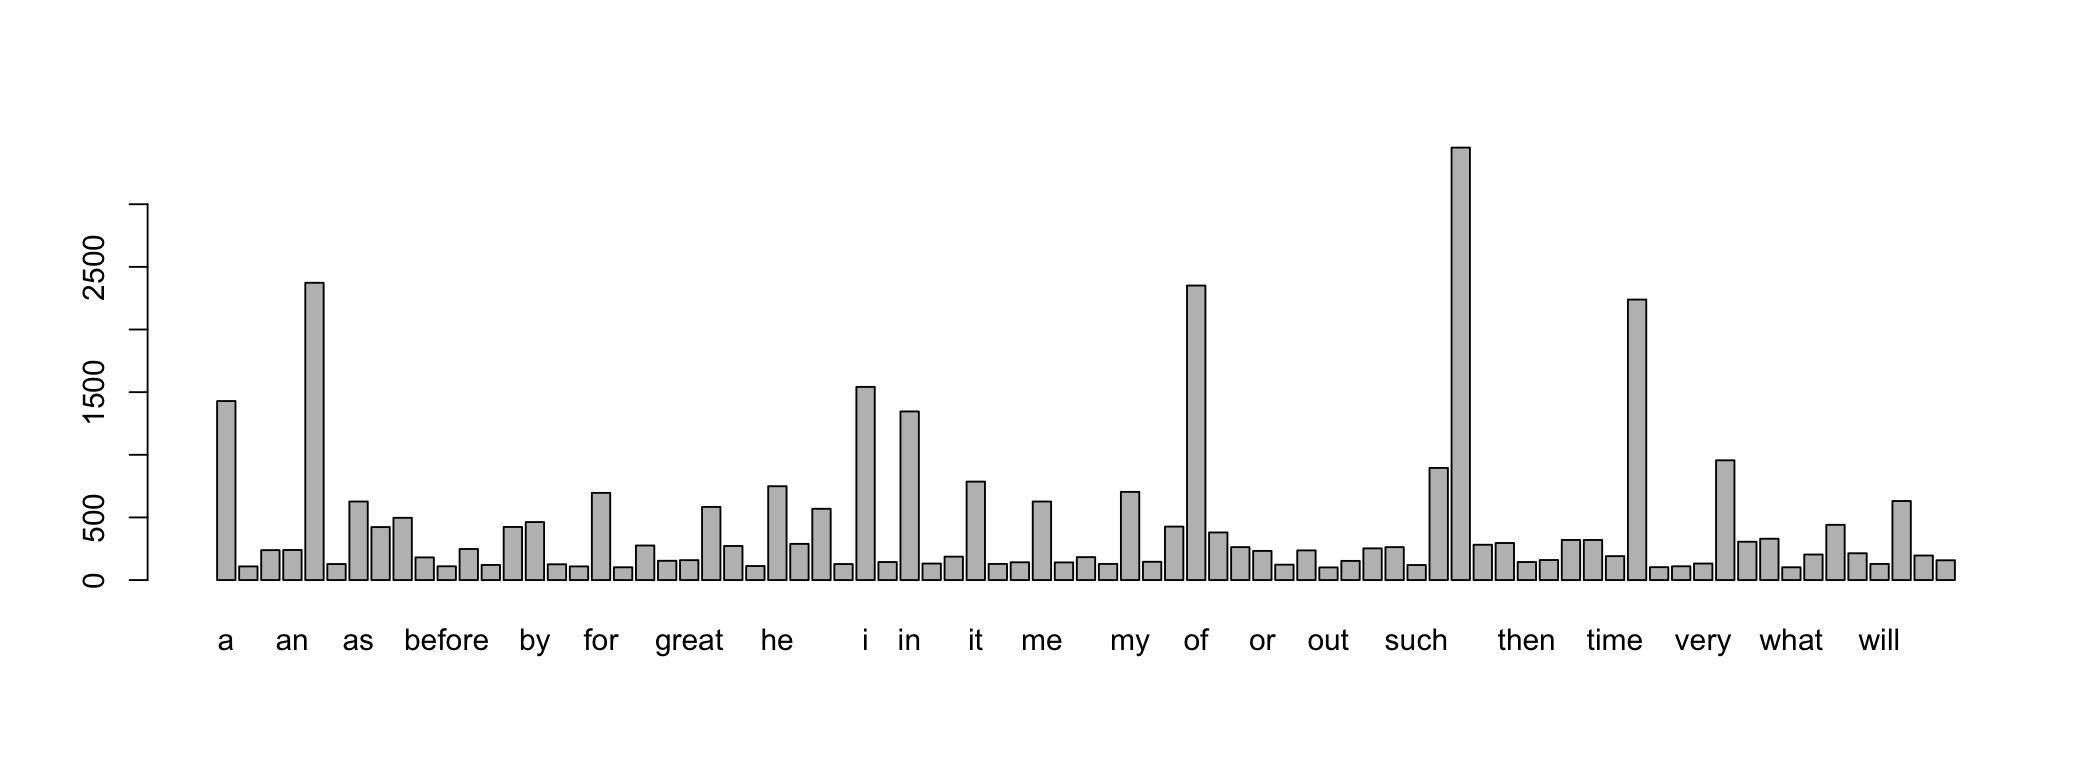
\includegraphics[width=170mm]{img/barplot_most_used_words}}
		\subfigure[Barplot of relevant words]{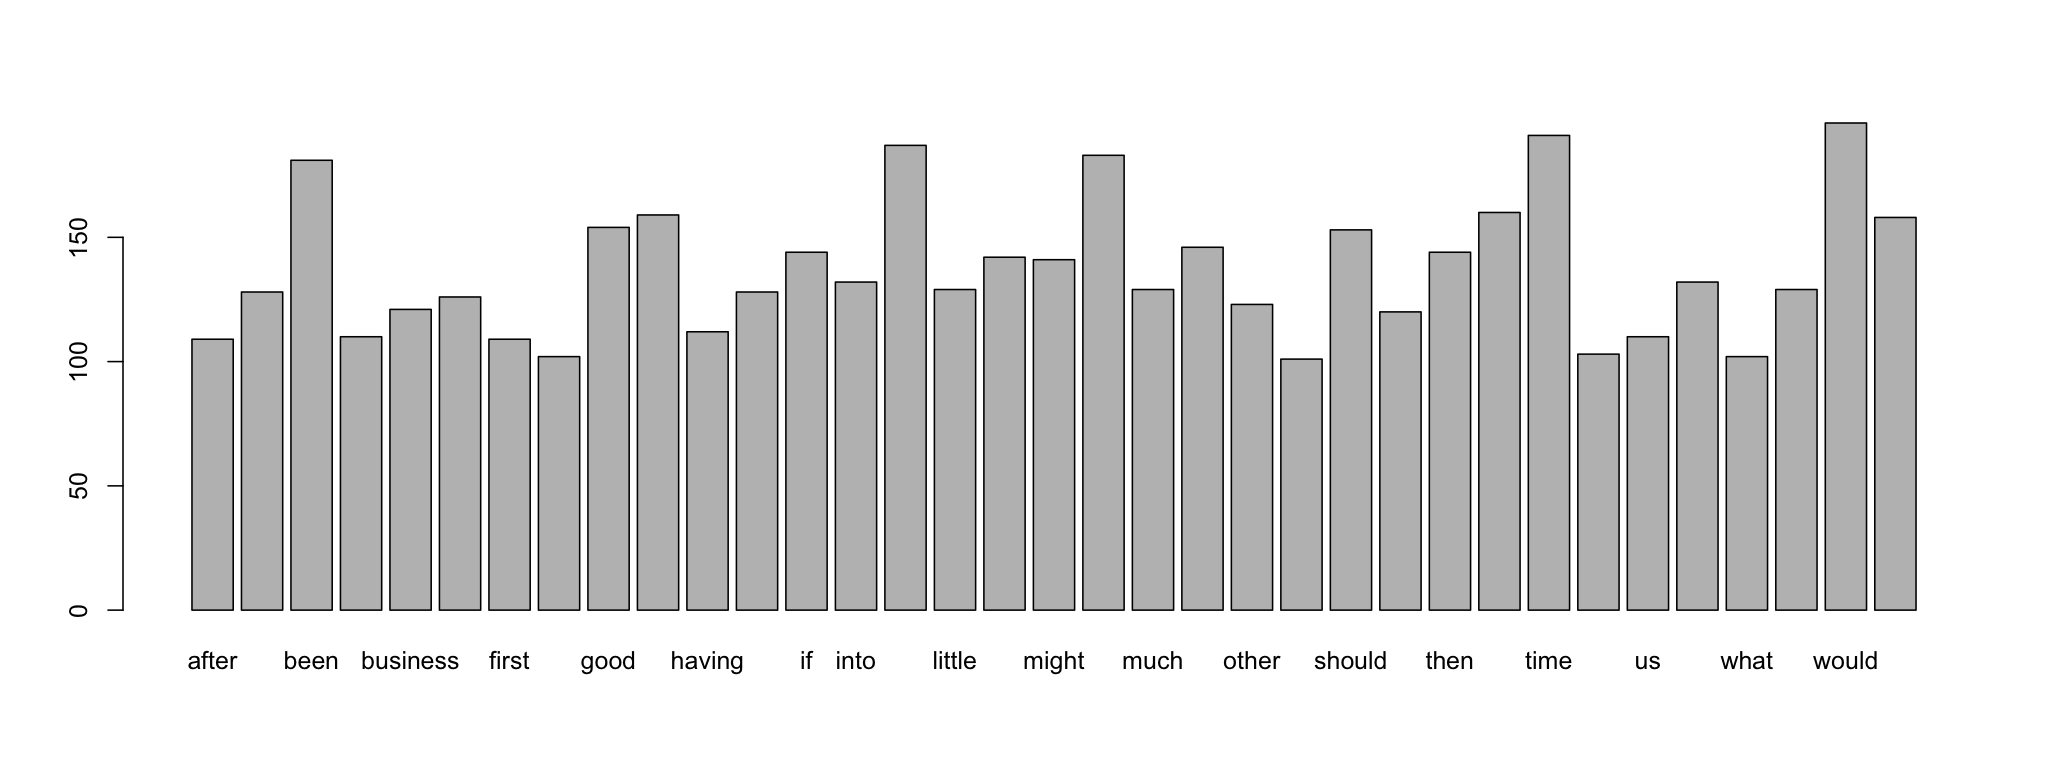
\includegraphics[width=170mm]{img/barplot_relevant_words}}
		
		\caption{Barplots of words present in the document} \label{fig:barplot_words1}
	\end{figure}

\begin{figure}
	\begin{center}
		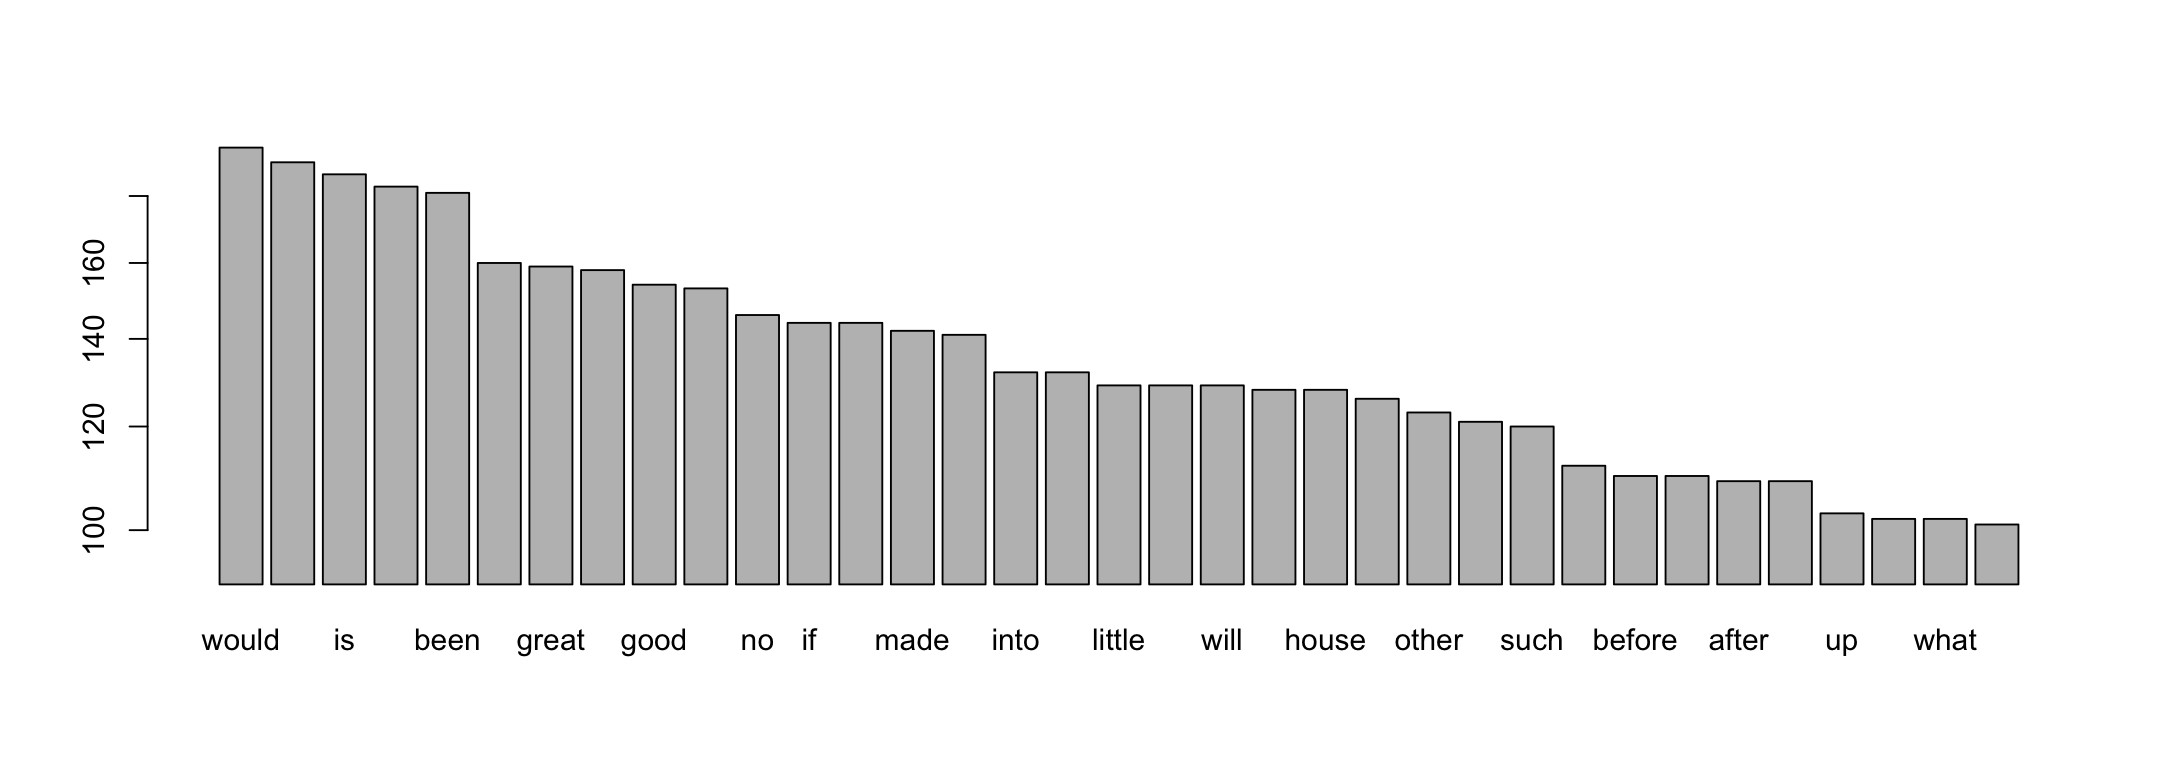
\includegraphics[scale=0.23]{img/barplot_relevant_words_ordered}
		\captionof{figure}{Barplot of relevant words  present in the document (sorted)}
		\label{fig:barplot_words2}
	\end{center}
\end{figure}
	
	Last, in Figure \ref{fig:barplot_places} it is generated a barplot, which shows an analysis of several places mentioned in the autobiography, and it can be seen as the most relevant ones in the life of this character. From this barplot most of the events related to Franklin took place in the city of Philadelphia.
	
	\begin{figure}
		\begin{center}
			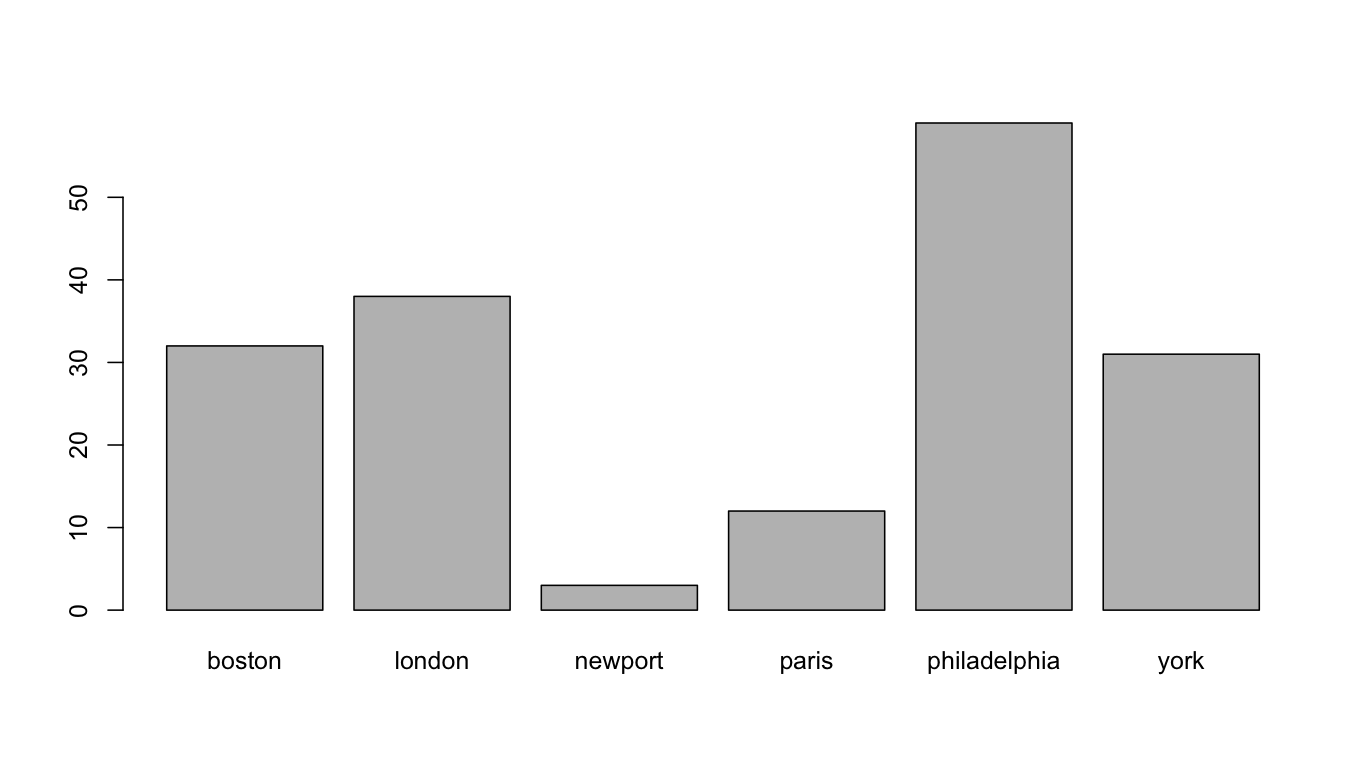
\includegraphics[scale=0.30]{img/barplot_places}
			\captionof{figure}{Barplot of relevant places mentioned in the document}
			\label{fig:barplot_places}
		\end{center}
	\end{figure}

\newpage

	\bibliography{assignment2}
	\bibliographystyle{plainnat}
	
\end{document}